\documentclass[tikz,border=0pt]{standalone}
% Estilo común de figuras y animaciones (mismos colores que la presentación)
% Compilar con XeLaTeX o LuaLaTeX (fuente TeX Gyre Heros); con pdfLaTeX usa Latin Modern Sans.
\usepackage{iftex}
\ifPDFTeX
  \usepackage[utf8]{inputenc}\usepackage[T1]{fontenc}\usepackage{lmodern}
  \renewcommand{\familydefault}{\sfdefault}
\else
  \usepackage{fontspec}\setmainfont{TeX Gyre Heros}\setsansfont{TeX Gyre Heros}
\fi
\usepackage{amssymb}
\usetikzlibrary{arrows.meta,positioning,calc,shapes.geometric,shadows,decorations.pathreplacing}
\definecolor{azul}{HTML}{1F3A5F}
\definecolor{acento}{HTML}{C0392B}
\definecolor{suave}{HTML}{EEF2F7}
\definecolor{gris}{HTML}{6B7280}
\definecolor{cOur}{HTML}{D62728}
\definecolor{cLib}{HTML}{1F77B4}
\definecolor{cWil}{HTML}{2CA02C}
\definecolor{cFol}{HTML}{FF7F0E}
\definecolor{cAnd}{HTML}{9467BD}
\definecolor{amarillo}{HTML}{F6C343}
\definecolor{verde}{HTML}{2E8B57}

% ---------- Iconos ----------
\providecommand{\iconscale}{1}
% \robot{pos}{color}{nombre}
\newcommand{\robot}[3]{%
  \begin{scope}[shift={#1}, scale=\iconscale, transform shape]
    \draw[#2, line width=0.8pt] (0,0.62) -- (0,0.78); \fill[#2] (0,0.8) circle (0.05);
    \draw[fill=#2!15, draw=#2, line width=0.8pt, rounded corners=2pt] (-0.3,0.25) rectangle (0.3,0.62);
    \fill[#2] (-0.13,0.45) circle (0.05); \fill[#2] (0.13,0.45) circle (0.05);
    \draw[#2, line width=0.6pt] (-0.1,0.33) -- (0.1,0.33);
    \draw[fill=#2!25, draw=#2, line width=0.8pt, rounded corners=2pt] (-0.24,-0.2) rectangle (0.24,0.22);
    \node[font=\tiny\bfseries, #2!70!black] at (0,-0.33) {#3};
  \end{scope}}
% \persona{pos}{color}{nombre}
\newcommand{\persona}[3]{%
  \begin{scope}[shift={#1}, scale=\iconscale, transform shape]
    \draw[fill=#2!20, draw=#2, line width=0.8pt] (0,0.5) circle (0.17);
    \draw[fill=#2!35, draw=#2, line width=0.8pt] (-0.27,-0.2) .. controls (-0.27,0.25) and (0.27,0.25) .. (0.27,-0.2) -- cycle;
    \node[font=\tiny\bfseries, #2!70!black] at (0,-0.33) {#3};
  \end{scope}}
% \libro{pos}{color}{texto}
\newcommand{\libro}[3]{%
  \begin{scope}[shift={#1}, scale=\iconscale, transform shape]
    \draw[fill=#2!25, draw=#2!80!black, line width=0.7pt, rounded corners=1pt] (-0.25,-0.32) rectangle (0.25,0.32);
    \fill[#2!80!black] (-0.25,-0.32) rectangle (-0.18,0.32);
    \node[font=\tiny\bfseries, align=center] at (0.035,0) {#3};
  \end{scope}}
% \letrero{pos}{texto principal}{tickets}
\newcommand{\letrero}[3]{%
  \begin{scope}[shift={#1}, scale=\iconscale, transform shape]
    \draw[fill=azul, draw=azul!60!black, rounded corners=2pt, line width=0.8pt] (-0.95,-0.32) rectangle (0.95,0.32);
    \foreach \i in {0,...,3} {\fill[cFol] (-0.85+\i*0.11,0.12) rectangle ++(0.08,0.12);}
    \foreach \i in {4,...,15} {\fill[amarillo!80] (-0.85+\i*0.11,0.12) rectangle ++(0.08,0.12);}
    \node[font=\tiny\bfseries, white] at (0,-0.12) {#2};
    \node[font=\tiny, cFol, anchor=south] at (-0.66,0.32) {#3};
  \end{scope}}
% \trituradora{pos}
\newcommand{\trituradora}[1]{%
  \begin{scope}[shift={#1}, scale=\iconscale, transform shape]
    \draw[fill=gris!25, draw=gris, line width=0.8pt] (-0.35,-0.25) rectangle (0.35,0.1);
    \draw[fill=gris!50, draw=gris] (-0.42,0.1) rectangle (0.42,0.2);
    \foreach \x in {-0.25,-0.12,0.01,0.14,0.27} {\draw[gris, line width=0.6pt] (\x,-0.25) -- (\x-0.03,-0.42);}
  \end{scope}}
% \ticket{pos}{color}
\newcommand{\ticket}[2]{%
  \begin{scope}[shift={#1}, scale=\iconscale, transform shape]
    \draw[fill=#2!30, draw=#2!80!black, line width=0.6pt] (-0.16,-0.09) -- (0.16,-0.09) -- (0.16,-0.03) arc (270:90:0.03) -- (0.16,0.09) -- (-0.16,0.09) -- (-0.16,0.03) arc (90:-90:0.03) -- cycle;
  \end{scope}}
% \contador{pos}{valor}{color}
\newcommand{\contador}[3]{%
  \node[scale=\iconscale, draw=#3, fill=white, line width=0.8pt, circle, inner sep=1.2pt, minimum size=0.42cm, font=\scriptsize\bfseries, text=#3] at #1 {#2};}

\renewcommand{\iconscale}{1.6}
\begin{document}
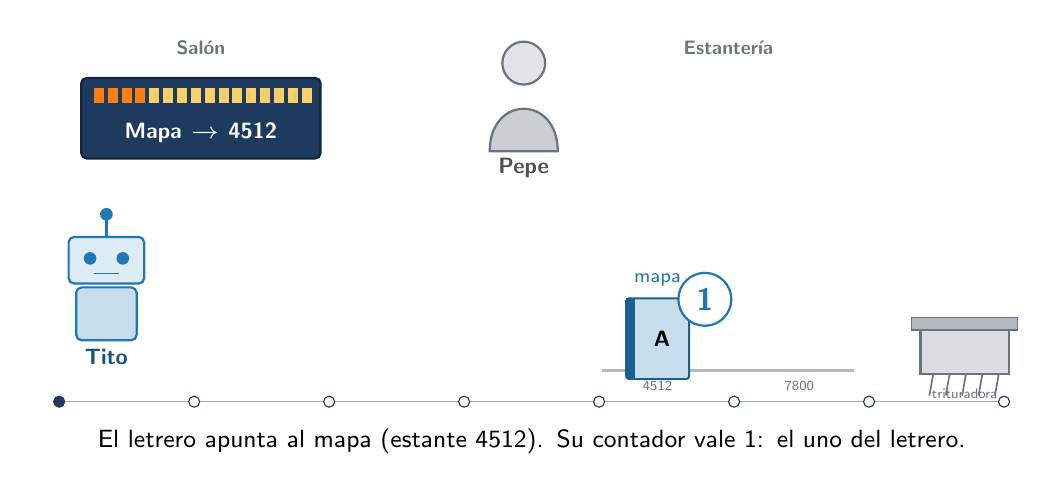
\begin{tikzpicture}
\useasboundingbox[fill=white] (0,0) rectangle (12.8,5.6);
\node[font=\scriptsize\bfseries, gris] at (2.2,5.35) {Salón};
\node[font=\scriptsize\bfseries, gris] at (8.9,5.35) {Estantería};
\draw[gris!50, line width=1pt] (7.3,1.25) -- (10.5,1.25);
\node[font=\tiny, gris] at (8.0,1.05) {4512};
\node[font=\tiny, gris] at (9.8,1.05) {7800};
\trituradora{(11.9,1.6)}
\node[font=\tiny, gris] at (11.9,0.95) {trituradora};
\letrero{(2.2,4.45)}{Mapa $\to$ 4512}{}
\libro{(8.0,1.65)}{cLib}{A}
\contador{(8.6,2.15)}{1}{cLib}
\node[font=\scriptsize, cLib] at (8.0,2.4) {mapa};
\robot{(1.0,1.95)}{cLib}{Tito}
\persona{(6.3,4.35)}{gris}{Pepe}
\draw[gris!60] (0.4,0.85) -- (12.4,0.85);
\draw[azul, fill=azul] (0.4,0.85) circle (0.07);
\draw[azul, fill=white] (2.1142857142857143,0.85) circle (0.07);
\draw[azul, fill=white] (3.8285714285714283,0.85) circle (0.07);
\draw[azul, fill=white] (5.542857142857144,0.85) circle (0.07);
\draw[azul, fill=white] (7.257142857142857,0.85) circle (0.07);
\draw[azul, fill=white] (8.971428571428572,0.85) circle (0.07);
\draw[azul, fill=white] (10.685714285714287,0.85) circle (0.07);
\draw[azul, fill=white] (12.4,0.85) circle (0.07);
\node[font=\small, text width=12.2cm, align=center, text=black] at (6.4,0.35) {El letrero apunta al mapa (estante 4512). Su contador vale 1: el uno del letrero.};
\end{tikzpicture}

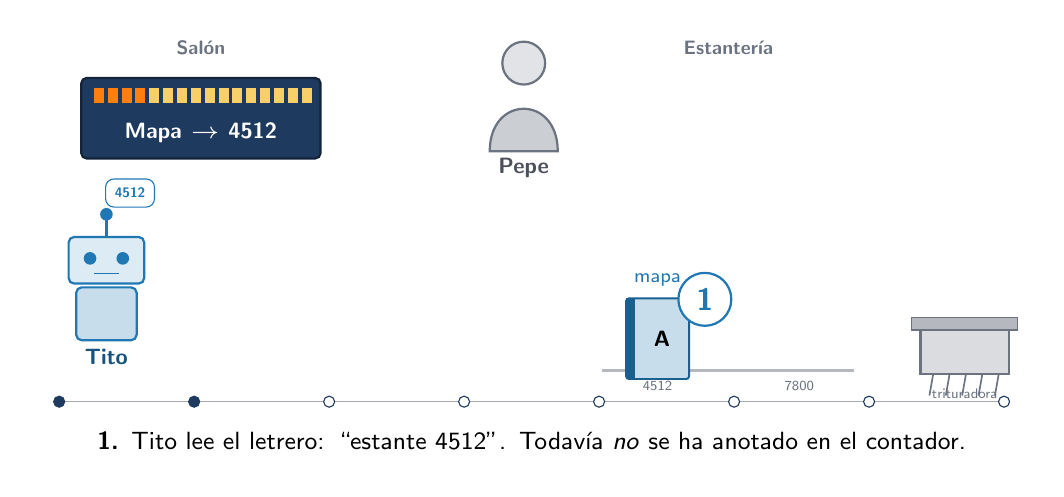
\begin{tikzpicture}
\useasboundingbox[fill=white] (0,0) rectangle (12.8,5.6);
\node[font=\scriptsize\bfseries, gris] at (2.2,5.35) {Salón};
\node[font=\scriptsize\bfseries, gris] at (8.9,5.35) {Estantería};
\draw[gris!50, line width=1pt] (7.3,1.25) -- (10.5,1.25);
\node[font=\tiny, gris] at (8.0,1.05) {4512};
\node[font=\tiny, gris] at (9.8,1.05) {7800};
\trituradora{(11.9,1.6)}
\node[font=\tiny, gris] at (11.9,0.95) {trituradora};
\letrero{(2.2,4.45)}{Mapa $\to$ 4512}{}
\libro{(8.0,1.65)}{cLib}{A}
\contador{(8.6,2.15)}{1}{cLib}
\node[font=\scriptsize, cLib] at (8.0,2.4) {mapa};
\robot{(1.0,1.95)}{cLib}{Tito}
\node[draw=cLib, fill=white, rounded corners=3pt, font=\tiny\bfseries, text=cLib] at (1.3,3.5) {4512};
\persona{(6.3,4.35)}{gris}{Pepe}
\draw[gris!60] (0.4,0.85) -- (12.4,0.85);
\draw[azul, fill=azul] (0.4,0.85) circle (0.07);
\draw[azul, fill=azul] (2.1142857142857143,0.85) circle (0.07);
\draw[azul, fill=white] (3.8285714285714283,0.85) circle (0.07);
\draw[azul, fill=white] (5.542857142857144,0.85) circle (0.07);
\draw[azul, fill=white] (7.257142857142857,0.85) circle (0.07);
\draw[azul, fill=white] (8.971428571428572,0.85) circle (0.07);
\draw[azul, fill=white] (10.685714285714287,0.85) circle (0.07);
\draw[azul, fill=white] (12.4,0.85) circle (0.07);
\node[font=\small, text width=12.2cm, align=center, text=black] at (6.4,0.35) {\textbf{1.} Tito lee el letrero: ``estante 4512''. Todavía \emph{no} se ha anotado en el contador.};
\end{tikzpicture}

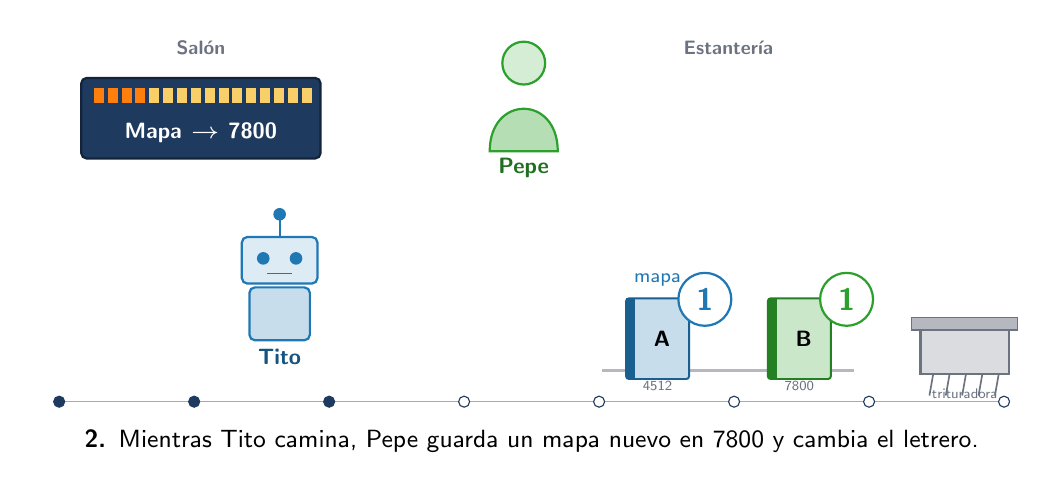
\begin{tikzpicture}
\useasboundingbox[fill=white] (0,0) rectangle (12.8,5.6);
\node[font=\scriptsize\bfseries, gris] at (2.2,5.35) {Salón};
\node[font=\scriptsize\bfseries, gris] at (8.9,5.35) {Estantería};
\draw[gris!50, line width=1pt] (7.3,1.25) -- (10.5,1.25);
\node[font=\tiny, gris] at (8.0,1.05) {4512};
\node[font=\tiny, gris] at (9.8,1.05) {7800};
\trituradora{(11.9,1.6)}
\node[font=\tiny, gris] at (11.9,0.95) {trituradora};
\letrero{(2.2,4.45)}{Mapa $\to$ 7800}{}
\libro{(9.8,1.65)}{cWil}{B}
\contador{(10.4,2.15)}{1}{cWil}
\libro{(8.0,1.65)}{cLib}{A}
\contador{(8.6,2.15)}{1}{cLib}
\node[font=\scriptsize, cLib] at (8.0,2.4) {mapa};
\robot{(3.2,1.95)}{cLib}{Tito}
\persona{(6.3,4.35)}{cWil}{Pepe}
\draw[gris!60] (0.4,0.85) -- (12.4,0.85);
\draw[azul, fill=azul] (0.4,0.85) circle (0.07);
\draw[azul, fill=azul] (2.1142857142857143,0.85) circle (0.07);
\draw[azul, fill=azul] (3.8285714285714283,0.85) circle (0.07);
\draw[azul, fill=white] (5.542857142857144,0.85) circle (0.07);
\draw[azul, fill=white] (7.257142857142857,0.85) circle (0.07);
\draw[azul, fill=white] (8.971428571428572,0.85) circle (0.07);
\draw[azul, fill=white] (10.685714285714287,0.85) circle (0.07);
\draw[azul, fill=white] (12.4,0.85) circle (0.07);
\node[font=\small, text width=12.2cm, align=center, text=black] at (6.4,0.35) {\textbf{2.} Mientras Tito camina, Pepe guarda un mapa nuevo en 7800 y cambia el letrero.};
\end{tikzpicture}

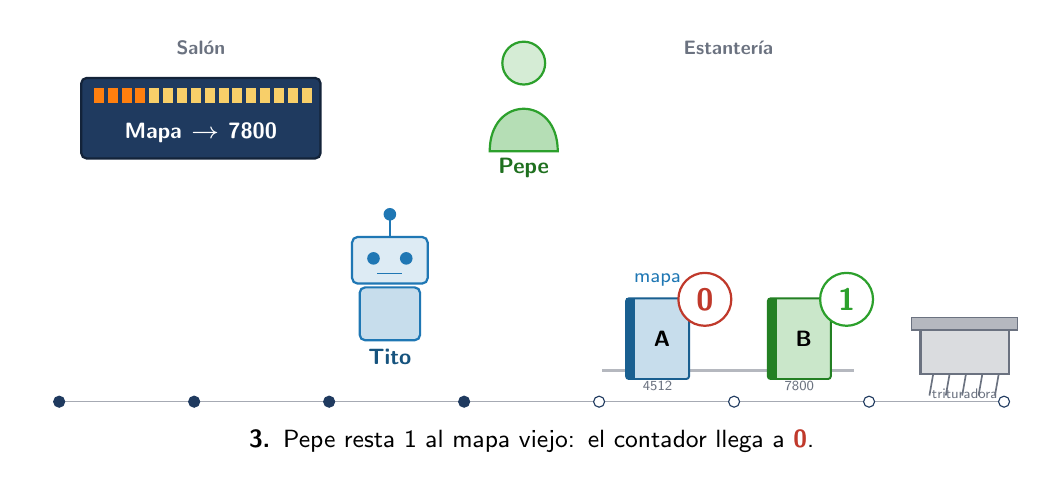
\begin{tikzpicture}
\useasboundingbox[fill=white] (0,0) rectangle (12.8,5.6);
\node[font=\scriptsize\bfseries, gris] at (2.2,5.35) {Salón};
\node[font=\scriptsize\bfseries, gris] at (8.9,5.35) {Estantería};
\draw[gris!50, line width=1pt] (7.3,1.25) -- (10.5,1.25);
\node[font=\tiny, gris] at (8.0,1.05) {4512};
\node[font=\tiny, gris] at (9.8,1.05) {7800};
\trituradora{(11.9,1.6)}
\node[font=\tiny, gris] at (11.9,0.95) {trituradora};
\letrero{(2.2,4.45)}{Mapa $\to$ 7800}{}
\libro{(9.8,1.65)}{cWil}{B}
\contador{(10.4,2.15)}{1}{cWil}
\libro{(8.0,1.65)}{cLib}{A}
\contador{(8.6,2.15)}{0}{acento}
\node[font=\scriptsize, cLib] at (8.0,2.4) {mapa};
\robot{(4.6,1.95)}{cLib}{Tito}
\persona{(6.3,4.35)}{cWil}{Pepe}
\draw[gris!60] (0.4,0.85) -- (12.4,0.85);
\draw[azul, fill=azul] (0.4,0.85) circle (0.07);
\draw[azul, fill=azul] (2.1142857142857143,0.85) circle (0.07);
\draw[azul, fill=azul] (3.8285714285714283,0.85) circle (0.07);
\draw[azul, fill=azul] (5.542857142857144,0.85) circle (0.07);
\draw[azul, fill=white] (7.257142857142857,0.85) circle (0.07);
\draw[azul, fill=white] (8.971428571428572,0.85) circle (0.07);
\draw[azul, fill=white] (10.685714285714287,0.85) circle (0.07);
\draw[azul, fill=white] (12.4,0.85) circle (0.07);
\node[font=\small, text width=12.2cm, align=center, text=black] at (6.4,0.35) {\textbf{3.} Pepe resta 1 al mapa viejo: el contador llega a \textcolor{acento}{\textbf{0}}.};
\end{tikzpicture}

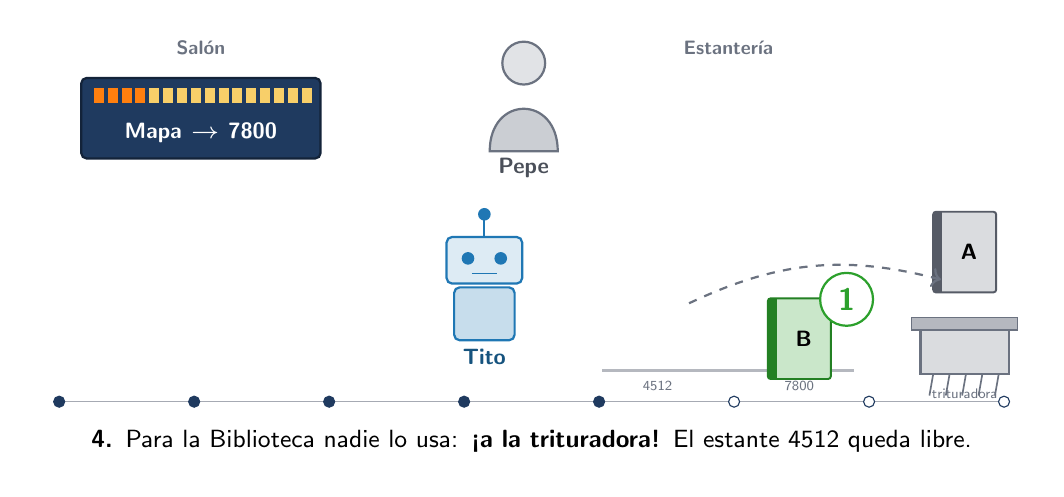
\begin{tikzpicture}
\useasboundingbox[fill=white] (0,0) rectangle (12.8,5.6);
\node[font=\scriptsize\bfseries, gris] at (2.2,5.35) {Salón};
\node[font=\scriptsize\bfseries, gris] at (8.9,5.35) {Estantería};
\draw[gris!50, line width=1pt] (7.3,1.25) -- (10.5,1.25);
\node[font=\tiny, gris] at (8.0,1.05) {4512};
\node[font=\tiny, gris] at (9.8,1.05) {7800};
\trituradora{(11.9,1.6)}
\node[font=\tiny, gris] at (11.9,0.95) {trituradora};
\letrero{(2.2,4.45)}{Mapa $\to$ 7800}{}
\libro{(9.8,1.65)}{cWil}{B}
\contador{(10.4,2.15)}{1}{cWil}
\libro{(11.9,2.75)}{gris}{A}
\draw[->, gris, thick, dashed] (8.4,2.1) to[bend left=20] (11.6,2.4);
\robot{(5.8,1.95)}{cLib}{Tito}
\persona{(6.3,4.35)}{gris}{Pepe}
\draw[gris!60] (0.4,0.85) -- (12.4,0.85);
\draw[azul, fill=azul] (0.4,0.85) circle (0.07);
\draw[azul, fill=azul] (2.1142857142857143,0.85) circle (0.07);
\draw[azul, fill=azul] (3.8285714285714283,0.85) circle (0.07);
\draw[azul, fill=azul] (5.542857142857144,0.85) circle (0.07);
\draw[azul, fill=azul] (7.257142857142857,0.85) circle (0.07);
\draw[azul, fill=white] (8.971428571428572,0.85) circle (0.07);
\draw[azul, fill=white] (10.685714285714287,0.85) circle (0.07);
\draw[azul, fill=white] (12.4,0.85) circle (0.07);
\node[font=\small, text width=12.2cm, align=center, text=black] at (6.4,0.35) {\textbf{4.} Para la Biblioteca nadie lo usa: \textbf{¡a la trituradora!} El estante 4512 queda libre.};
\end{tikzpicture}

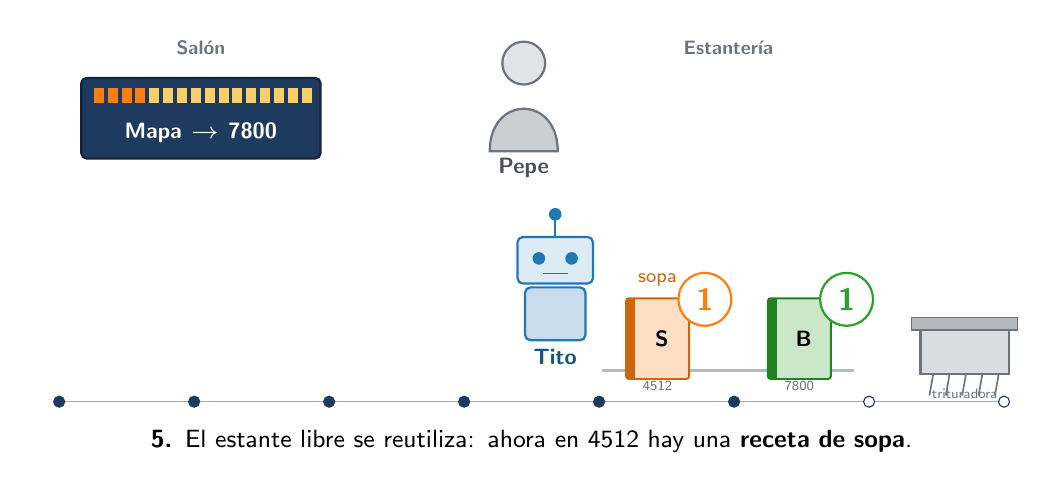
\begin{tikzpicture}
\useasboundingbox[fill=white] (0,0) rectangle (12.8,5.6);
\node[font=\scriptsize\bfseries, gris] at (2.2,5.35) {Salón};
\node[font=\scriptsize\bfseries, gris] at (8.9,5.35) {Estantería};
\draw[gris!50, line width=1pt] (7.3,1.25) -- (10.5,1.25);
\node[font=\tiny, gris] at (8.0,1.05) {4512};
\node[font=\tiny, gris] at (9.8,1.05) {7800};
\trituradora{(11.9,1.6)}
\node[font=\tiny, gris] at (11.9,0.95) {trituradora};
\letrero{(2.2,4.45)}{Mapa $\to$ 7800}{}
\libro{(9.8,1.65)}{cWil}{B}
\contador{(10.4,2.15)}{1}{cWil}
\libro{(8.0,1.65)}{cFol}{S}
\contador{(8.6,2.15)}{1}{cFol}
\node[font=\scriptsize, cFol!80!black] at (8.0,2.4) {sopa};
\robot{(6.7,1.95)}{cLib}{Tito}
\persona{(6.3,4.35)}{gris}{Pepe}
\draw[gris!60] (0.4,0.85) -- (12.4,0.85);
\draw[azul, fill=azul] (0.4,0.85) circle (0.07);
\draw[azul, fill=azul] (2.1142857142857143,0.85) circle (0.07);
\draw[azul, fill=azul] (3.8285714285714283,0.85) circle (0.07);
\draw[azul, fill=azul] (5.542857142857144,0.85) circle (0.07);
\draw[azul, fill=azul] (7.257142857142857,0.85) circle (0.07);
\draw[azul, fill=azul] (8.971428571428572,0.85) circle (0.07);
\draw[azul, fill=white] (10.685714285714287,0.85) circle (0.07);
\draw[azul, fill=white] (12.4,0.85) circle (0.07);
\node[font=\small, text width=12.2cm, align=center, text=black] at (6.4,0.35) {\textbf{5.} El estante libre se reutiliza: ahora en 4512 hay una \textbf{receta de sopa}.};
\end{tikzpicture}

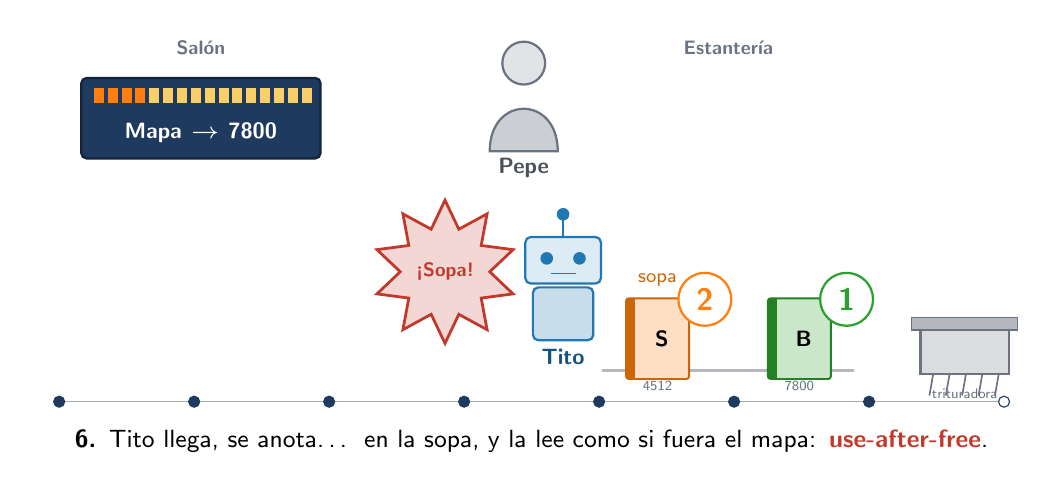
\begin{tikzpicture}
\useasboundingbox[fill=white] (0,0) rectangle (12.8,5.6);
\node[font=\scriptsize\bfseries, gris] at (2.2,5.35) {Salón};
\node[font=\scriptsize\bfseries, gris] at (8.9,5.35) {Estantería};
\draw[gris!50, line width=1pt] (7.3,1.25) -- (10.5,1.25);
\node[font=\tiny, gris] at (8.0,1.05) {4512};
\node[font=\tiny, gris] at (9.8,1.05) {7800};
\trituradora{(11.9,1.6)}
\node[font=\tiny, gris] at (11.9,0.95) {trituradora};
\letrero{(2.2,4.45)}{Mapa $\to$ 7800}{}
\libro{(9.8,1.65)}{cWil}{B}
\contador{(10.4,2.15)}{1}{cWil}
\libro{(8.0,1.65)}{cFol}{S}
\contador{(8.6,2.15)}{2}{cFol}
\node[font=\scriptsize, cFol!80!black] at (8.0,2.4) {sopa};
\robot{(6.8,1.95)}{cLib}{Tito}
\persona{(6.3,4.35)}{gris}{Pepe}
\node[star, star points=10, star point ratio=1.6, fill=acento!20, draw=acento, line width=1pt, font=\scriptsize\bfseries, text=acento, inner sep=1pt] at (5.3,2.5) {¡Sopa!};
\draw[gris!60] (0.4,0.85) -- (12.4,0.85);
\draw[azul, fill=azul] (0.4,0.85) circle (0.07);
\draw[azul, fill=azul] (2.1142857142857143,0.85) circle (0.07);
\draw[azul, fill=azul] (3.8285714285714283,0.85) circle (0.07);
\draw[azul, fill=azul] (5.542857142857144,0.85) circle (0.07);
\draw[azul, fill=azul] (7.257142857142857,0.85) circle (0.07);
\draw[azul, fill=azul] (8.971428571428572,0.85) circle (0.07);
\draw[azul, fill=azul] (10.685714285714287,0.85) circle (0.07);
\draw[azul, fill=white] (12.4,0.85) circle (0.07);
\node[font=\small, text width=12.2cm, align=center, text=black] at (6.4,0.35) {\textbf{6.} Tito llega, se anota\ldots{} en la sopa, y la lee como si fuera el mapa: \textcolor{acento}{\textbf{use-after-free}}.};
\end{tikzpicture}

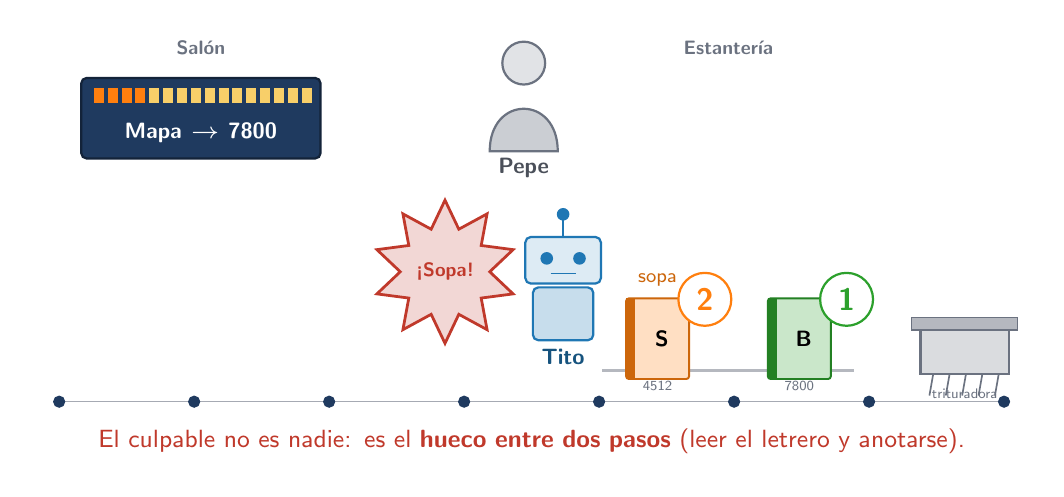
\begin{tikzpicture}
\useasboundingbox[fill=white] (0,0) rectangle (12.8,5.6);
\node[font=\scriptsize\bfseries, gris] at (2.2,5.35) {Salón};
\node[font=\scriptsize\bfseries, gris] at (8.9,5.35) {Estantería};
\draw[gris!50, line width=1pt] (7.3,1.25) -- (10.5,1.25);
\node[font=\tiny, gris] at (8.0,1.05) {4512};
\node[font=\tiny, gris] at (9.8,1.05) {7800};
\trituradora{(11.9,1.6)}
\node[font=\tiny, gris] at (11.9,0.95) {trituradora};
\letrero{(2.2,4.45)}{Mapa $\to$ 7800}{}
\libro{(9.8,1.65)}{cWil}{B}
\contador{(10.4,2.15)}{1}{cWil}
\libro{(8.0,1.65)}{cFol}{S}
\contador{(8.6,2.15)}{2}{cFol}
\node[font=\scriptsize, cFol!80!black] at (8.0,2.4) {sopa};
\robot{(6.8,1.95)}{cLib}{Tito}
\persona{(6.3,4.35)}{gris}{Pepe}
\node[star, star points=10, star point ratio=1.6, fill=acento!20, draw=acento, line width=1pt, font=\scriptsize\bfseries, text=acento, inner sep=1pt] at (5.3,2.5) {¡Sopa!};
\draw[gris!60] (0.4,0.85) -- (12.4,0.85);
\draw[azul, fill=azul] (0.4,0.85) circle (0.07);
\draw[azul, fill=azul] (2.1142857142857143,0.85) circle (0.07);
\draw[azul, fill=azul] (3.8285714285714283,0.85) circle (0.07);
\draw[azul, fill=azul] (5.542857142857144,0.85) circle (0.07);
\draw[azul, fill=azul] (7.257142857142857,0.85) circle (0.07);
\draw[azul, fill=azul] (8.971428571428572,0.85) circle (0.07);
\draw[azul, fill=azul] (10.685714285714287,0.85) circle (0.07);
\draw[azul, fill=azul] (12.4,0.85) circle (0.07);
\node[font=\small, text width=12.2cm, align=center, text=acento] at (6.4,0.35) {El culpable no es nadie: es el \textbf{hueco entre dos pasos} (leer el letrero y anotarse).};
\end{tikzpicture}
\end{document}
